\chapter{DHCP (Dynamic Host Configuration
Protocol)}\label{dhcp-dynamic-host-configuration-protocol}

\section{The Purpose of DHCP}\label{the-purpose-of-dhcp}

\begin{itemize}
\tightlist
\item
  DHCP is used to allow HOSTS to automatically / dynamically learn
  various aspects of their NETWORK configuration; without MANUAL /
  STATIC configuration
\item
  It is an ESSENTIAL part of modern NETWORKS

  \begin{itemize}
  \tightlist
  \item
    When you connect a phone / laptop to WiFi, do you ask your NETWORK
    admin which IP ADDRESS, SUBNET MASK, DEFAULT GATEWAY, etc the phone
    / laptop should use ?
  \end{itemize}
\item
  Typically used for CLIENT devices (workstations, phones, etc)
\item
  DEVICES (such as ROUTERS, SERVERS, etc) are usually MANUALLY
  configured
\item
  In small NETWORKS (such as Home NETWORKS), the ROUTER typically acts
  as the DHCP SERVER for HOSTS in the LAN
\item
  In LARGE NETWORKS, the DHCP SERVER is usually a Windows / Linux SERVER
\end{itemize}

\section{Basic Functions of DHCP}\label{basic-functions-of-dhcp}

\begin{figure}
\centering
\pandocbounded{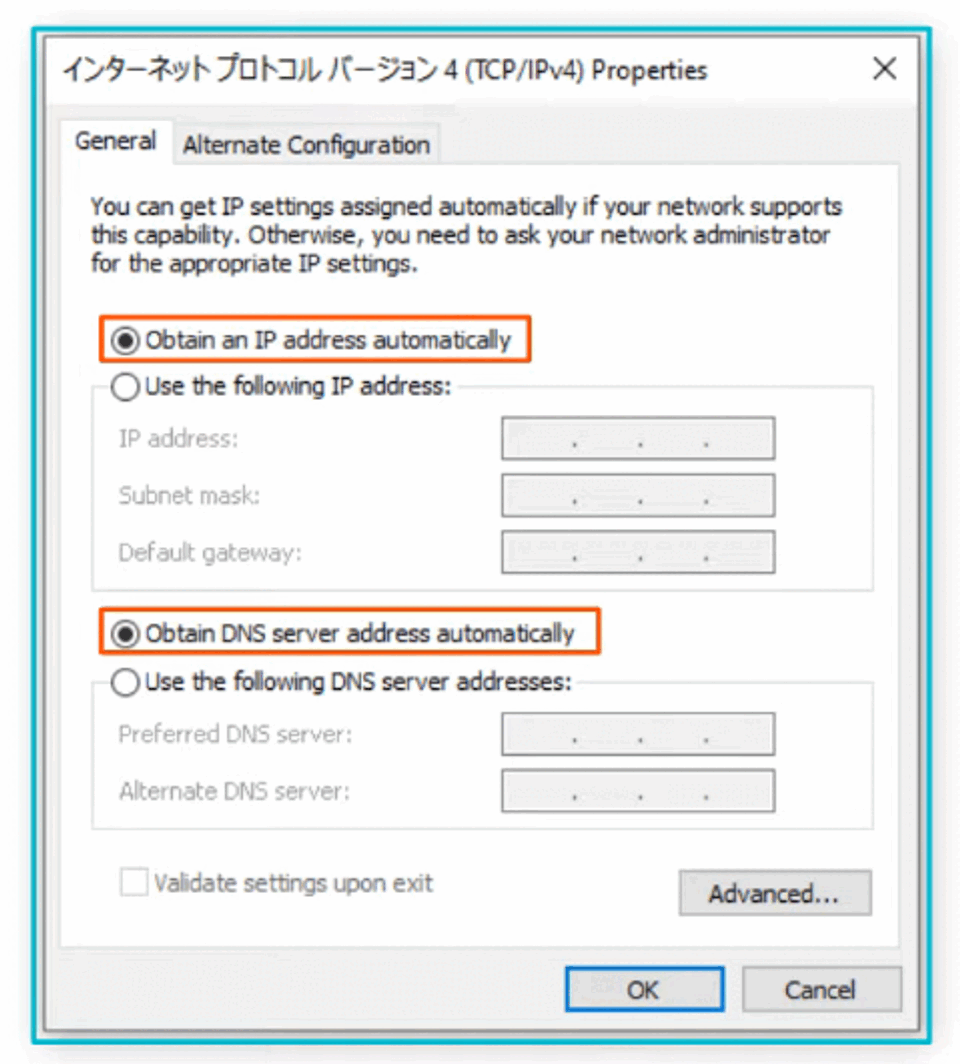
\includegraphics[keepaspectratio,alt={image}]{images/40-dhcp/img-001.png}}
\end{figure}

\begin{figure}
\centering
\pandocbounded{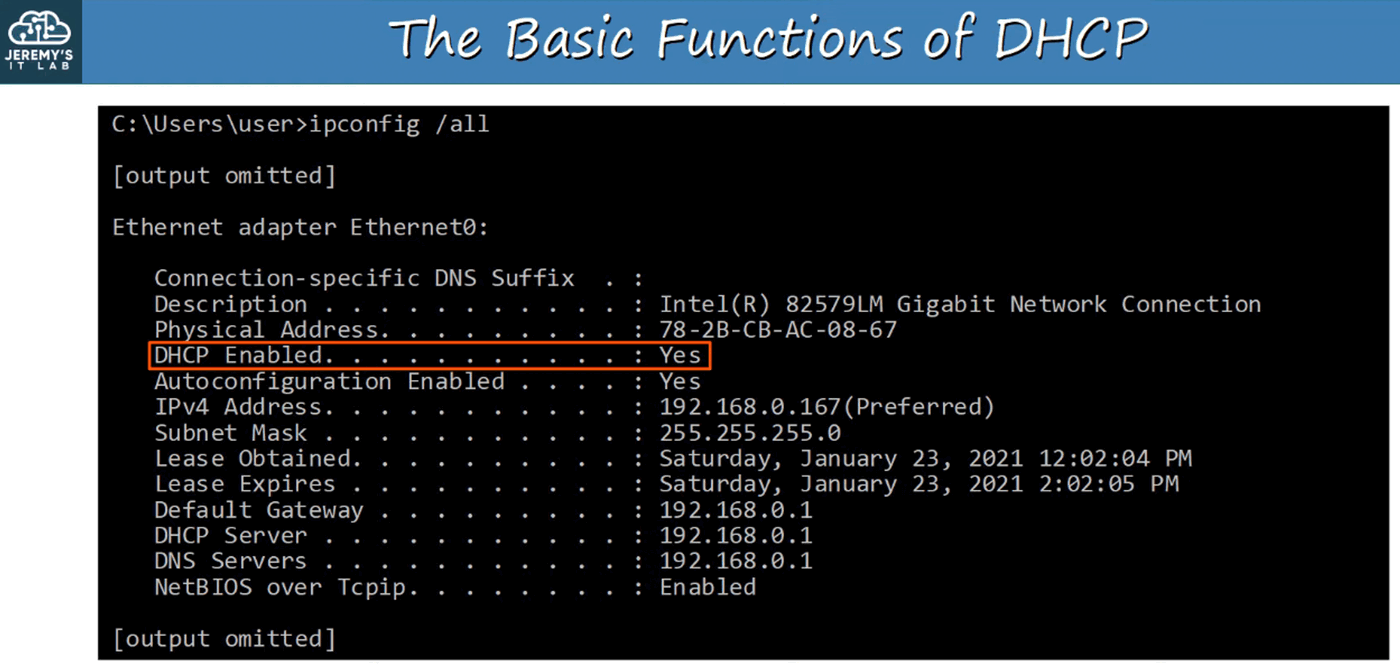
\includegraphics[keepaspectratio,alt={image}]{images/40-dhcp/img-002.png}}
\end{figure}

\begin{figure}
\centering
\pandocbounded{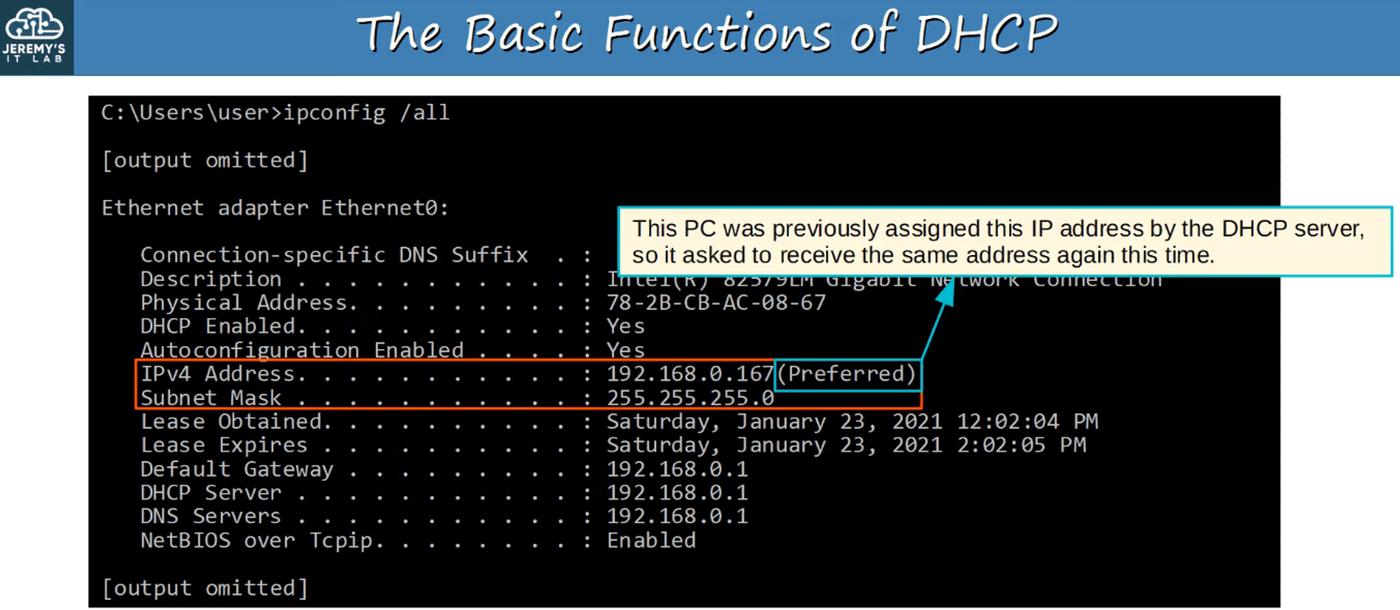
\includegraphics[keepaspectratio,alt={image}]{images/40-dhcp/img-003.png}}
\end{figure}

\begin{figure}
\centering
\pandocbounded{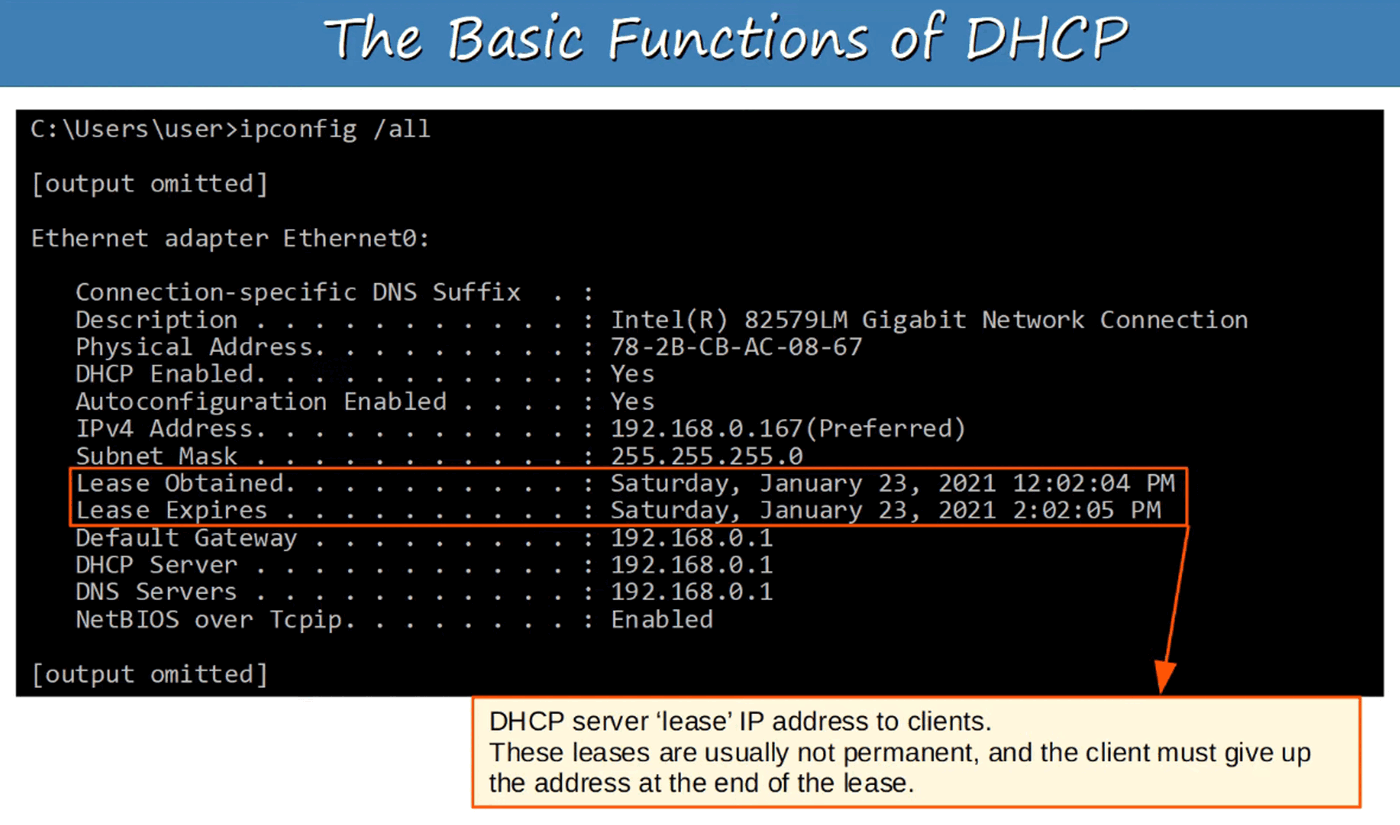
\includegraphics[keepaspectratio,alt={image}]{images/40-dhcp/img-004.png}}
\end{figure}

\begin{figure}
\centering
\pandocbounded{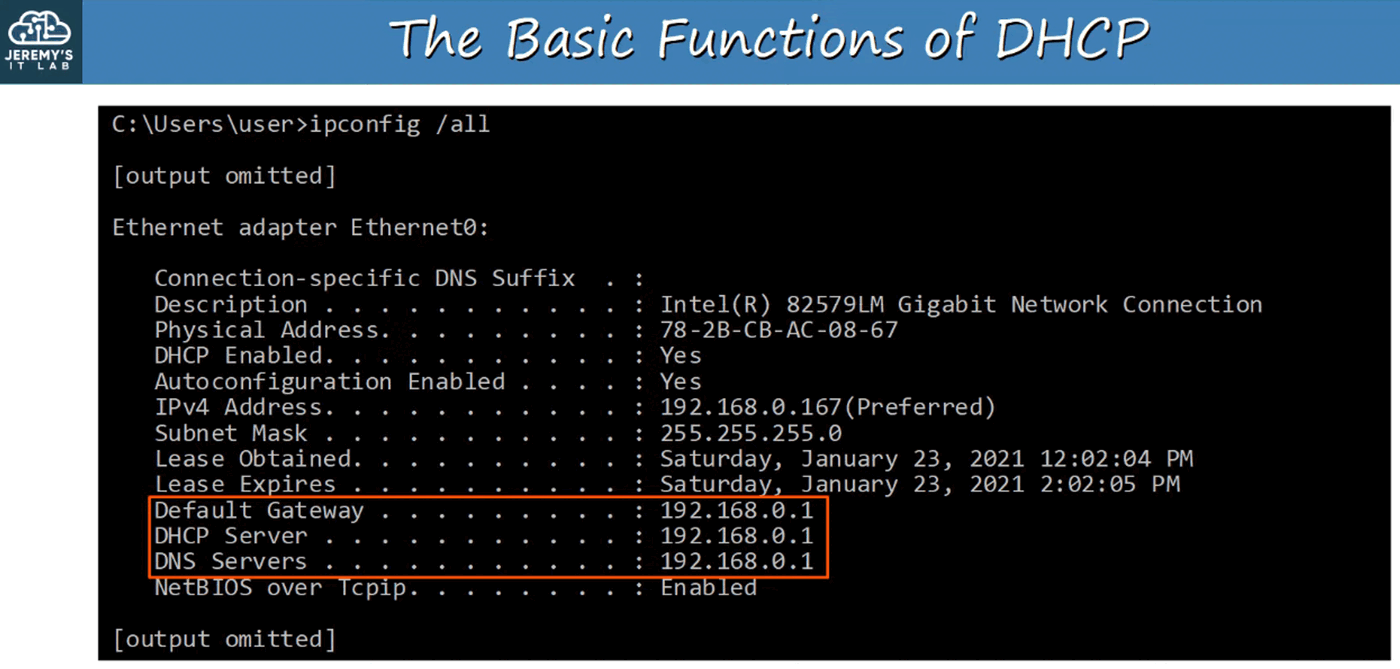
\includegraphics[keepaspectratio,alt={image}]{images/40-dhcp/img-005.png}}
\end{figure}

Note: ALL the IPs are the same because this is Jeremy's Home ROUTER (it
provides all these services)

Command \passthrough{\lstinline!ipconfig /release!}

\begin{figure}
\centering
\pandocbounded{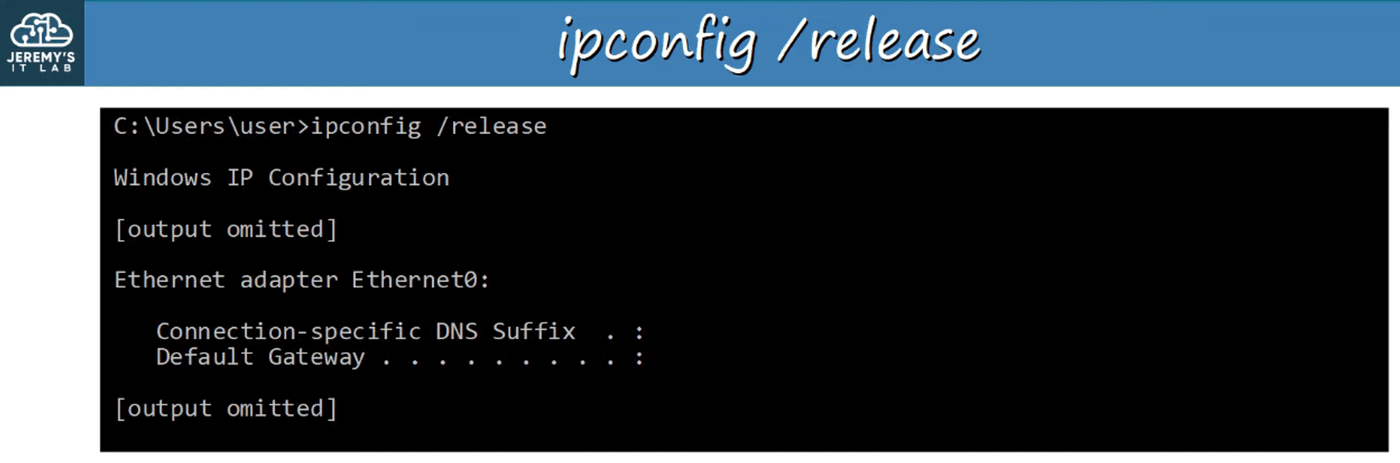
\includegraphics[keepaspectratio,alt={image}]{images/40-dhcp/img-006.png}}
\end{figure}

\begin{figure}
\centering
\pandocbounded{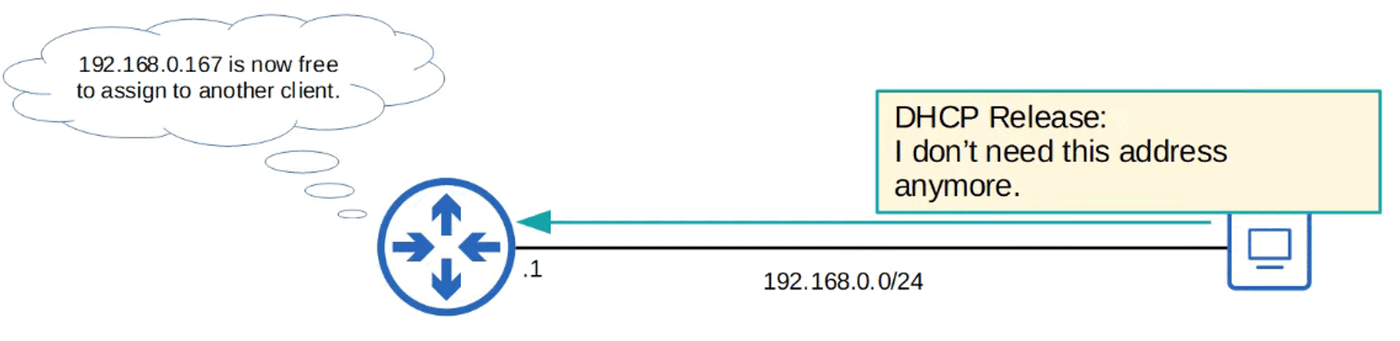
\includegraphics[keepaspectratio,alt={image}]{images/40-dhcp/img-007.png}}
\end{figure}

Wireshark capture of the \passthrough{\lstinline!ipconfig /release!}
mechanism

\begin{figure}
\centering
\pandocbounded{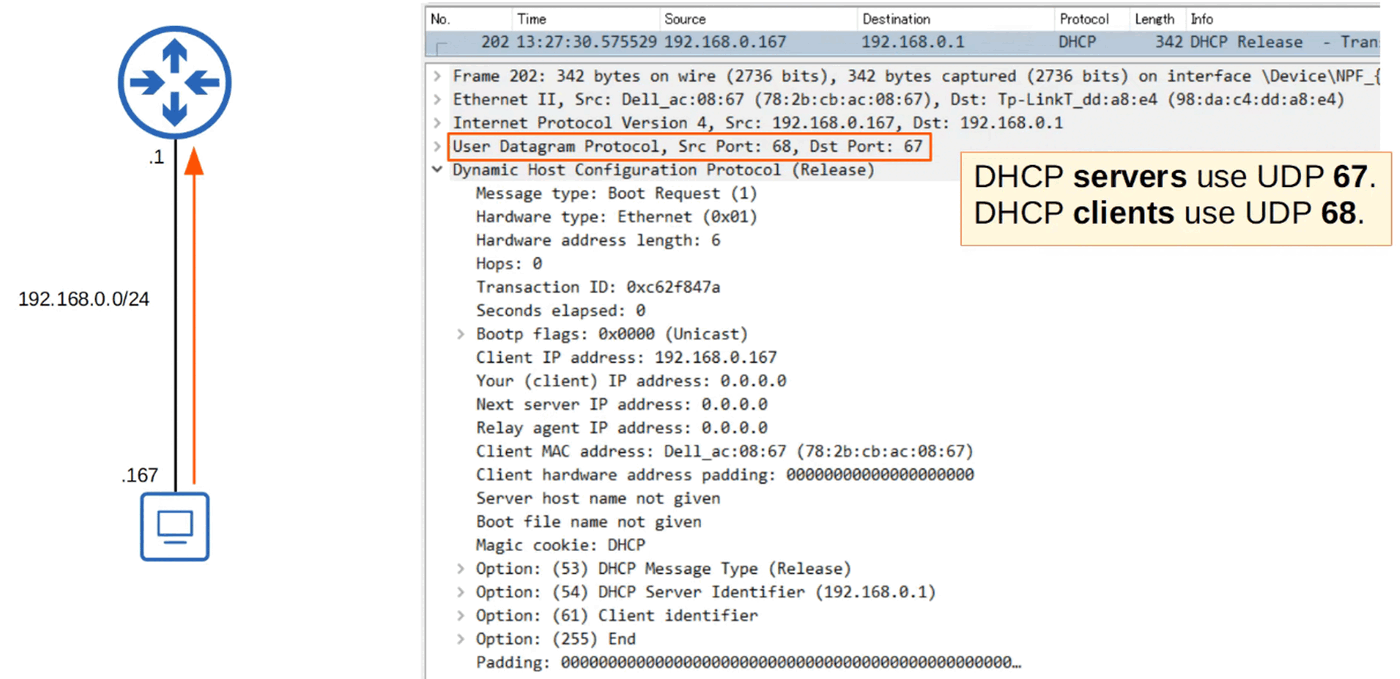
\includegraphics[keepaspectratio,alt={image}]{images/40-dhcp/img-008.png}}
\end{figure}

\begin{figure}
\centering
\pandocbounded{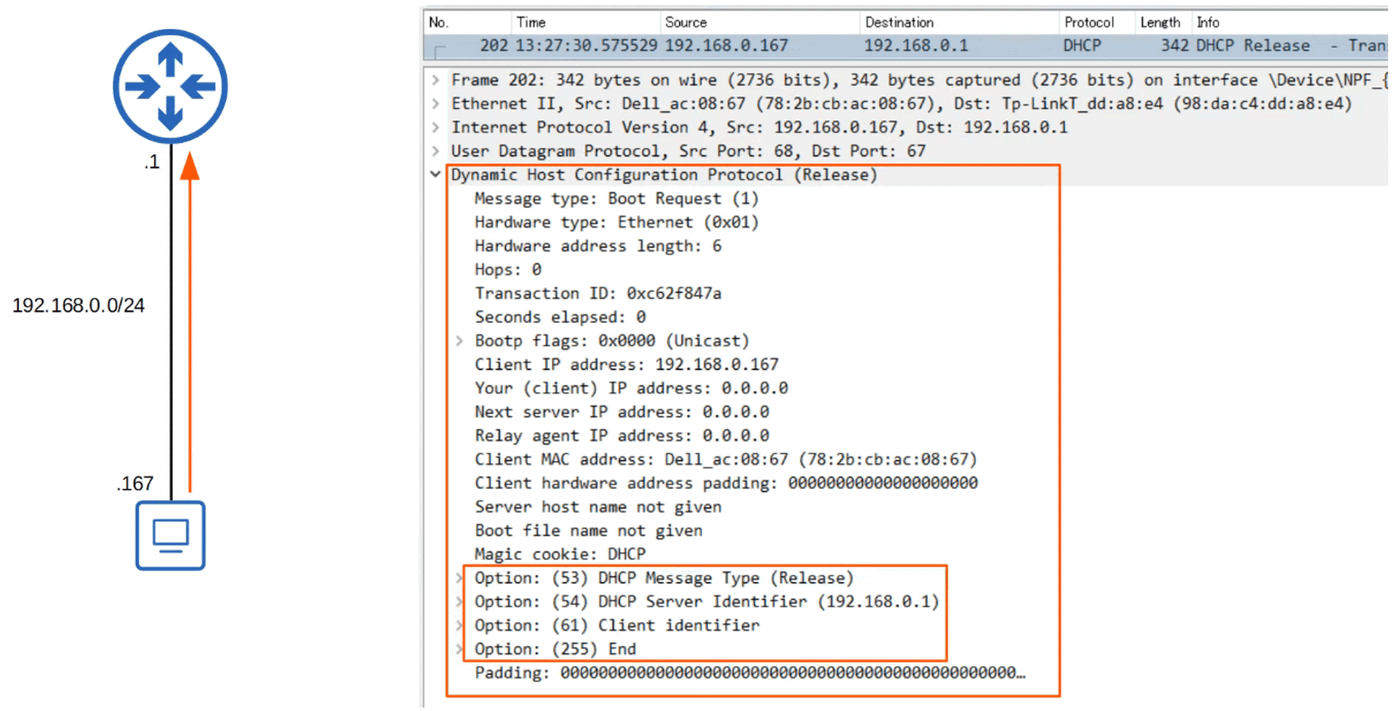
\includegraphics[keepaspectratio,alt={image}]{images/40-dhcp/img-009.png}}
\end{figure}

Command \passthrough{\lstinline!ipconfig /renew!}

\begin{figure}
\centering
\pandocbounded{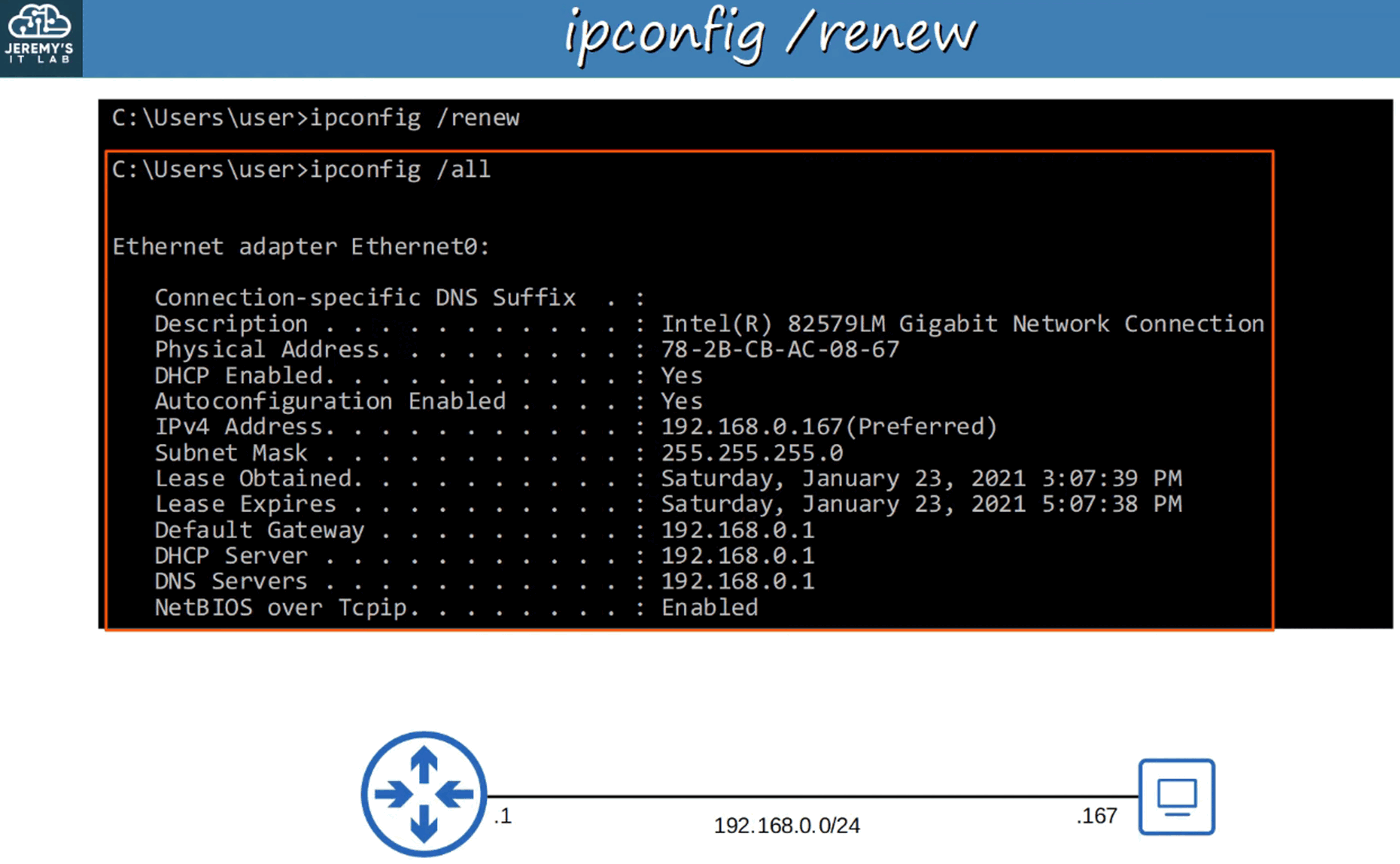
\includegraphics[keepaspectratio,alt={image}]{images/40-dhcp/img-010.png}}
\end{figure}

Renewing Process has FOUR messages:

\begin{figure}
\centering
\pandocbounded{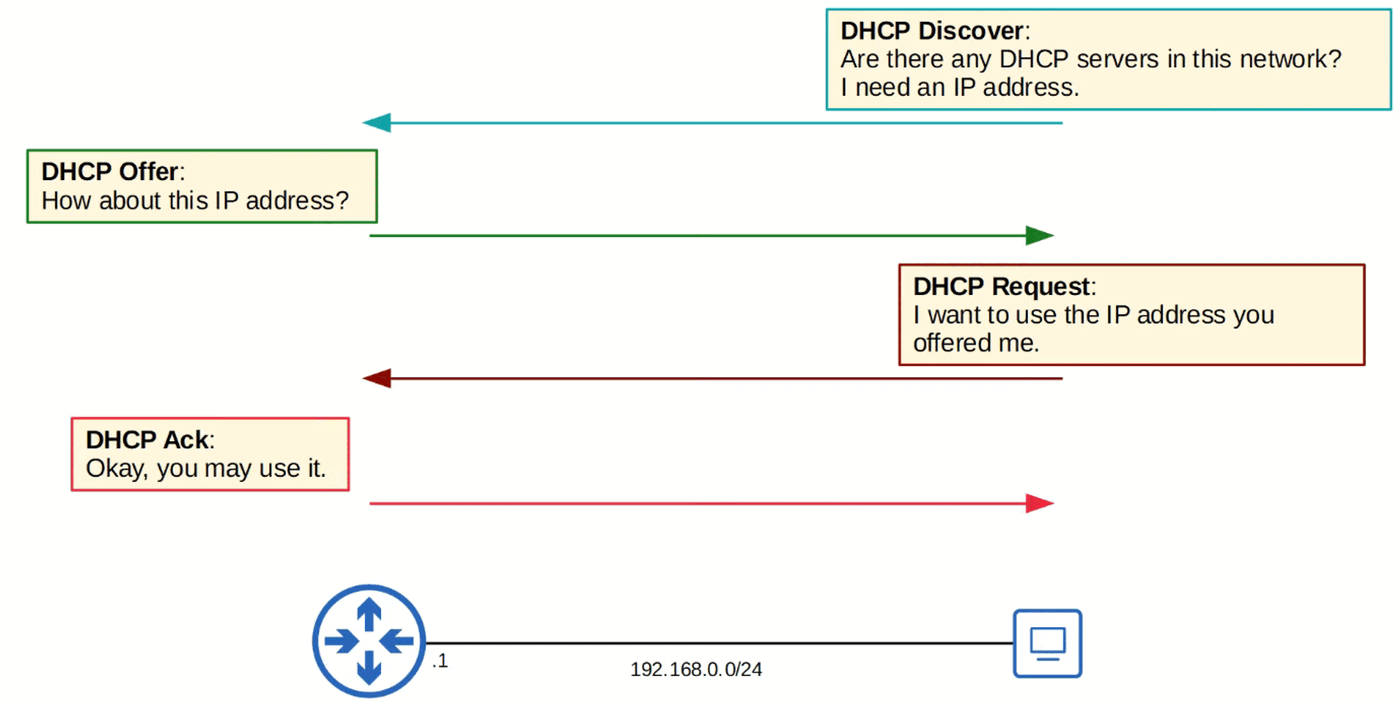
\includegraphics[keepaspectratio,alt={image}]{images/40-dhcp/img-011.png}}
\end{figure}

\begin{enumerate}
\def\labelenumi{\arabic{enumi})}
\tightlist
\item
  DHCP DISCOVER
\end{enumerate}

\begin{itemize}
\tightlist
\item
  Are there any DHCP Servers in this NETWORK? I need an IP ADDRESS ?
\end{itemize}

\begin{figure}
\centering
\pandocbounded{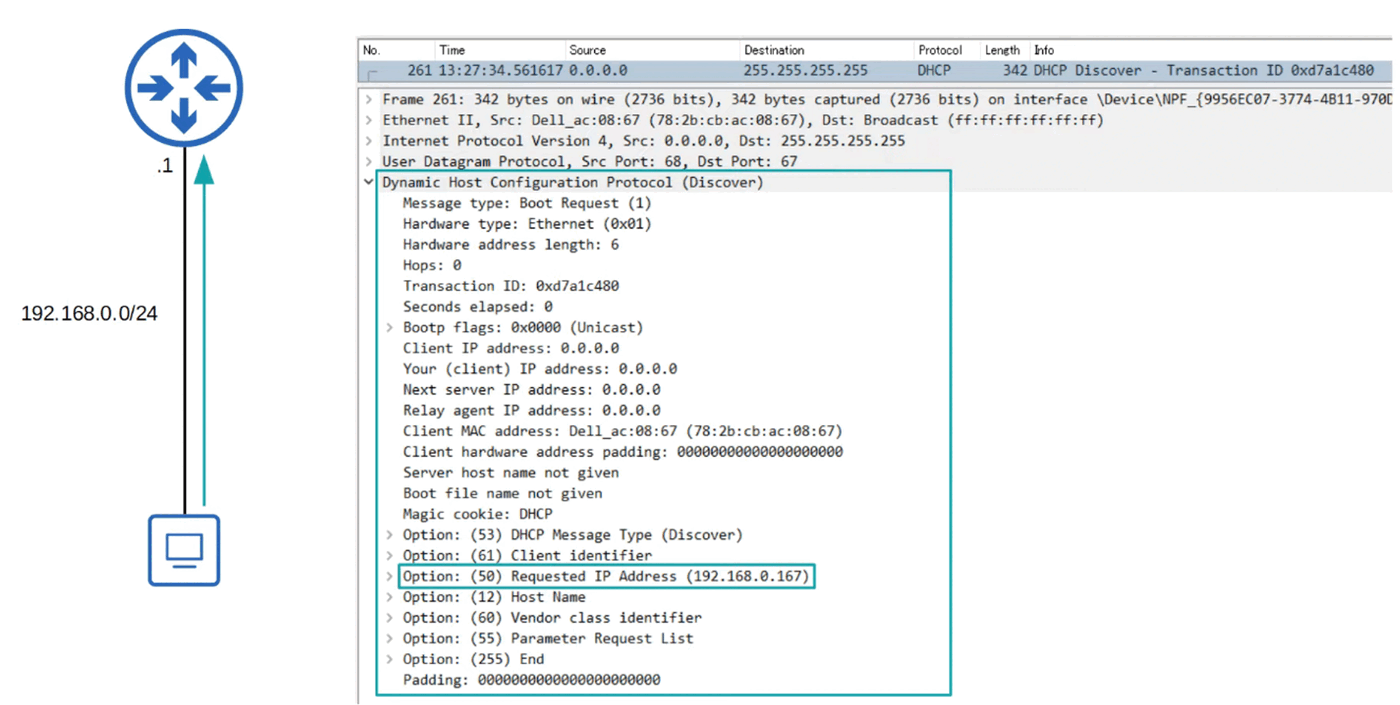
\includegraphics[keepaspectratio,alt={image}]{images/40-dhcp/img-012.png}}
\end{figure}

NOTE the use of DHCP Reserved Ports 67 and 68

\begin{enumerate}
\def\labelenumi{\arabic{enumi})}
\setcounter{enumi}{1}
\tightlist
\item
  DHCP OFFER:
\end{enumerate}

\begin{itemize}
\tightlist
\item
  How about THIS IP ADDRESS ?
\end{itemize}

\begin{figure}
\centering
\pandocbounded{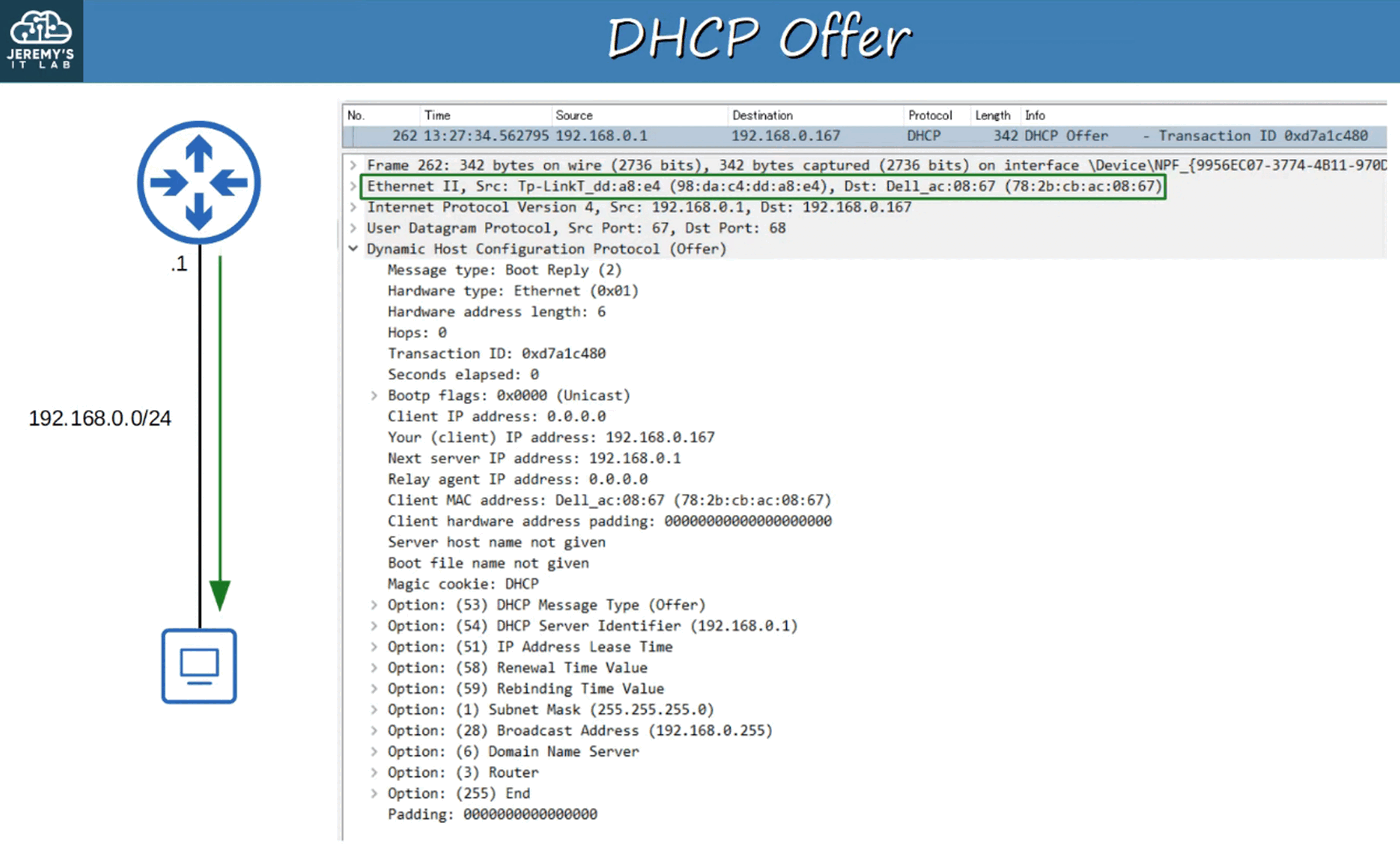
\includegraphics[keepaspectratio,alt={image}]{images/40-dhcp/img-013.png}}
\end{figure}

\begin{itemize}
\tightlist
\item
  The DHCP OFFER message can be either BROADCAST or UNICAST
\item
  NOTE OPTIONS at the bottom : Message Type, Server ID, Lease Time,
  Subnet, etc.
\end{itemize}

\begin{enumerate}
\def\labelenumi{\arabic{enumi})}
\setcounter{enumi}{2}
\tightlist
\item
  DHCP REQUEST
\end{enumerate}

\begin{itemize}
\tightlist
\item
  I want to use the IP ADDRESS that was offered
\end{itemize}

\begin{figure}
\centering
\pandocbounded{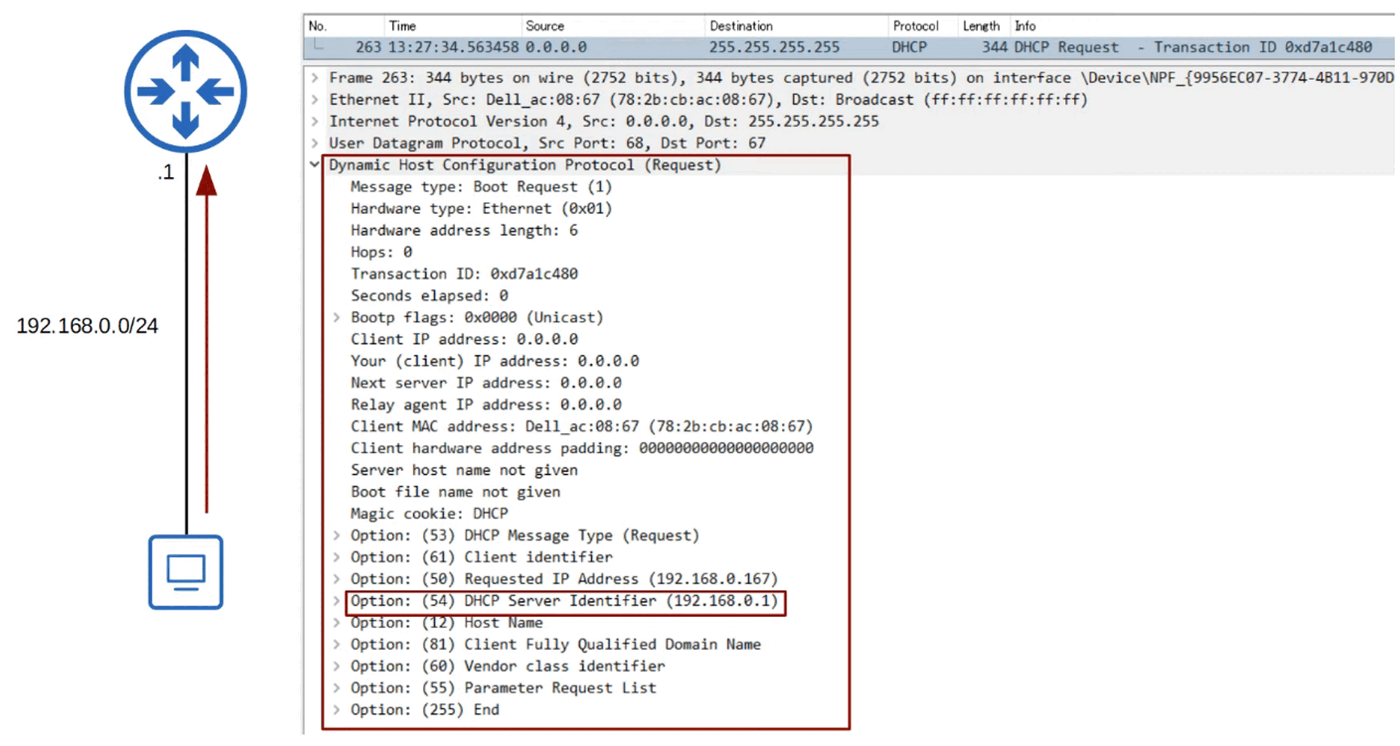
\includegraphics[keepaspectratio,alt={image}]{images/40-dhcp/img-014.png}}
\end{figure}

\begin{enumerate}
\def\labelenumi{\arabic{enumi})}
\setcounter{enumi}{3}
\tightlist
\item
  DHCP ACK
\end{enumerate}

\begin{itemize}
\tightlist
\item
  Okay! You may use THAT ADDRESS
\end{itemize}

\begin{figure}
\centering
\pandocbounded{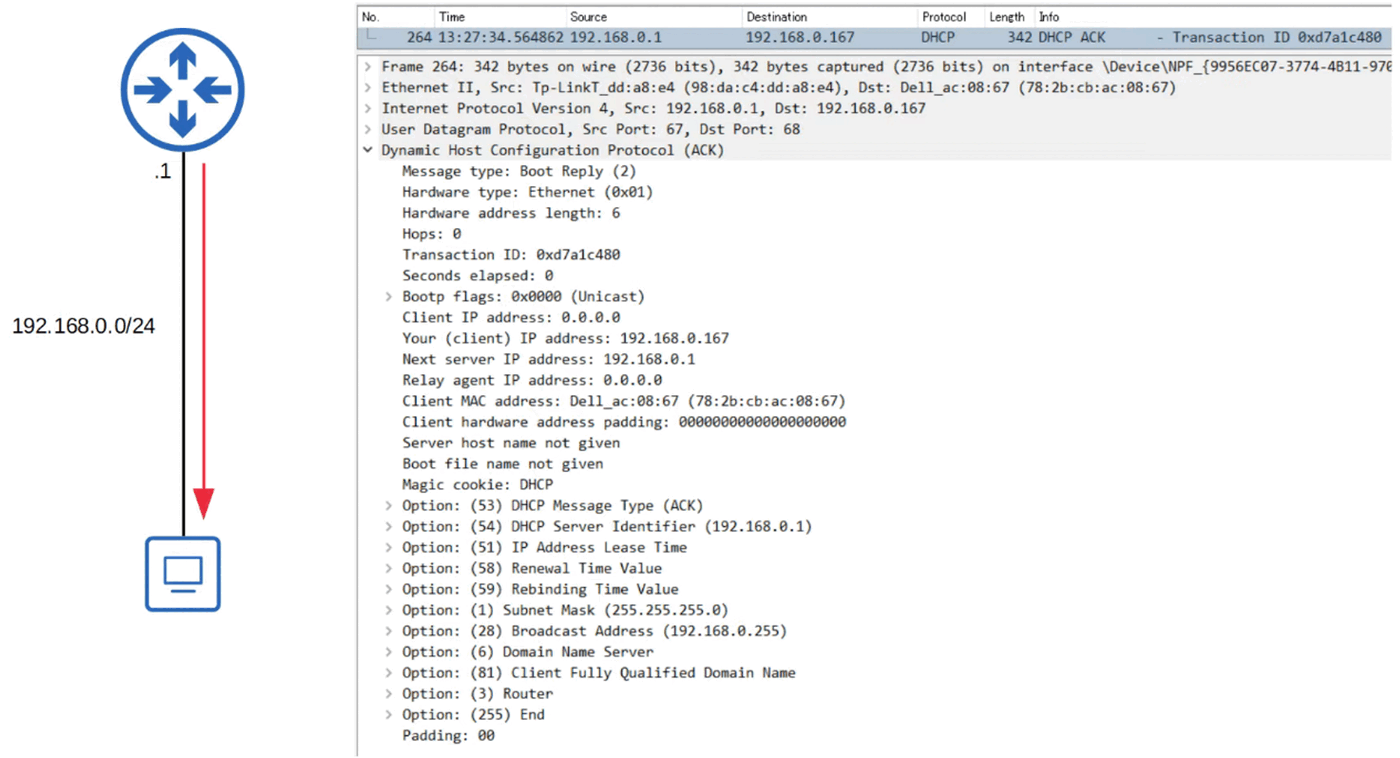
\includegraphics[keepaspectratio,alt={image}]{images/40-dhcp/img-015.png}}
\end{figure}

\section{DHCP Renew Process Summary}\label{dhcp-renew-process-summary}

\begin{figure}
\centering
\pandocbounded{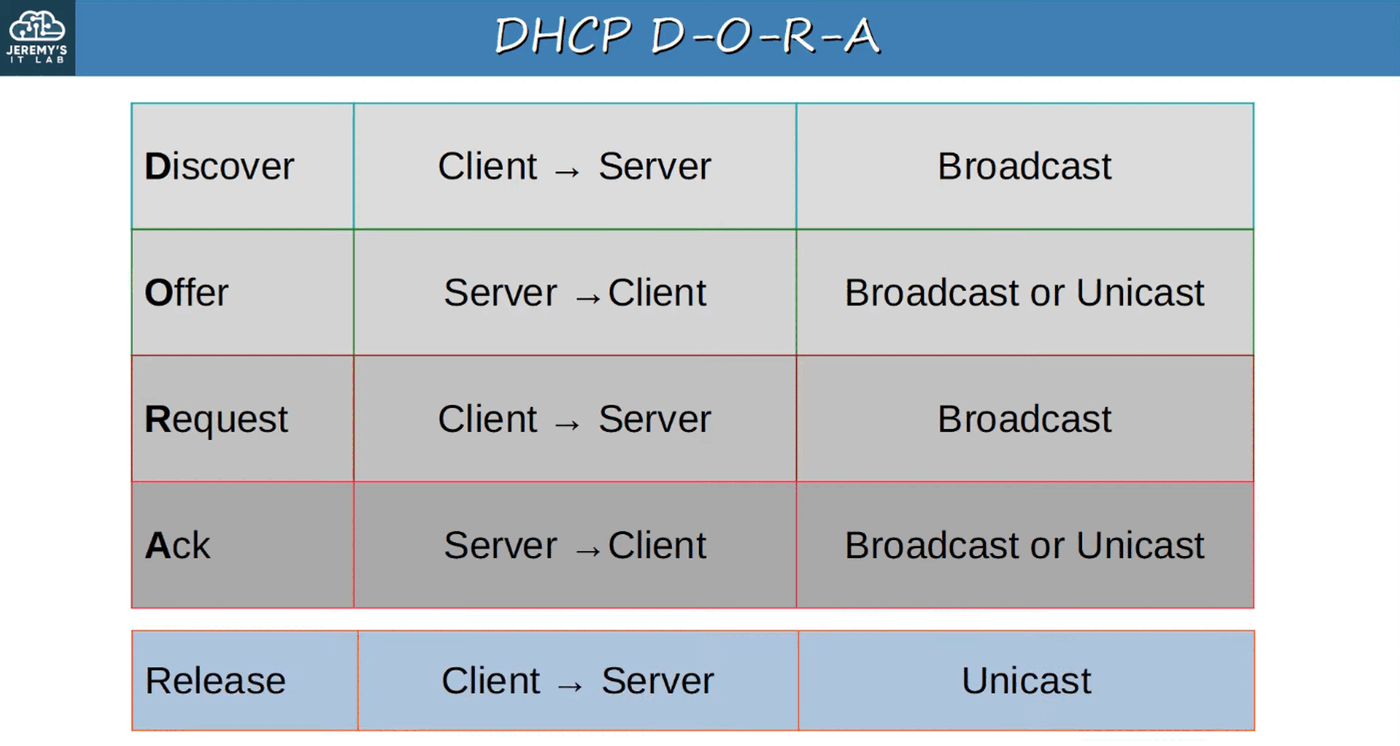
\includegraphics[keepaspectratio,alt={image}]{images/40-dhcp/img-016.png}}
\end{figure}

\section{DHCP Relay}\label{dhcp-relay}

\begin{itemize}
\tightlist
\item
  Some NETWORK engineers might choose to configure each ROUTER to act as
  the DHCP SERVER for its connected LANS
\item
  However, large enterprises often choose to use a CENTRALIZED DHCP
  SERVER
\item
  If the SERVER is centralized, it won't receive the DHCP CLIENTS'
  Broadcast DHCP messages
\item
  To FIX this, you can configure a ROUTER to act as a DHCP RELAY AGENT
\item
  The ROUTER will forward the clients' Broadcast DHCP messages to the
  remote DHCP SERVER as a Unicast messages
\end{itemize}

\begin{figure}
\centering
\pandocbounded{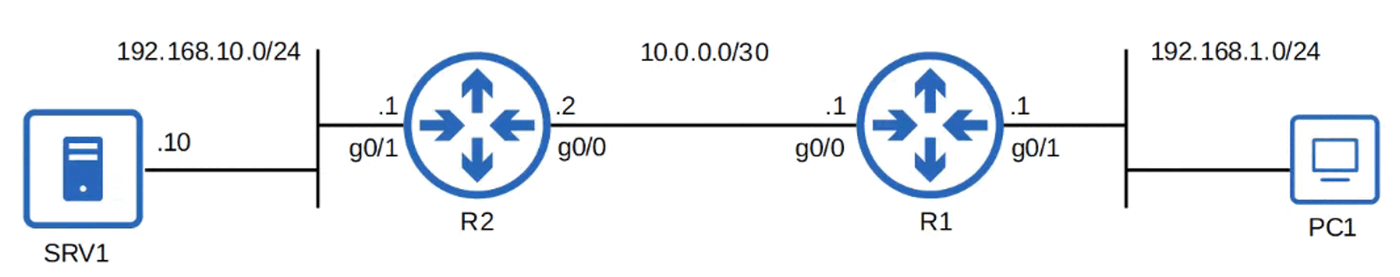
\includegraphics[keepaspectratio,alt={image}]{images/40-dhcp/img-017.png}}
\end{figure}

\begin{figure}
\centering
\pandocbounded{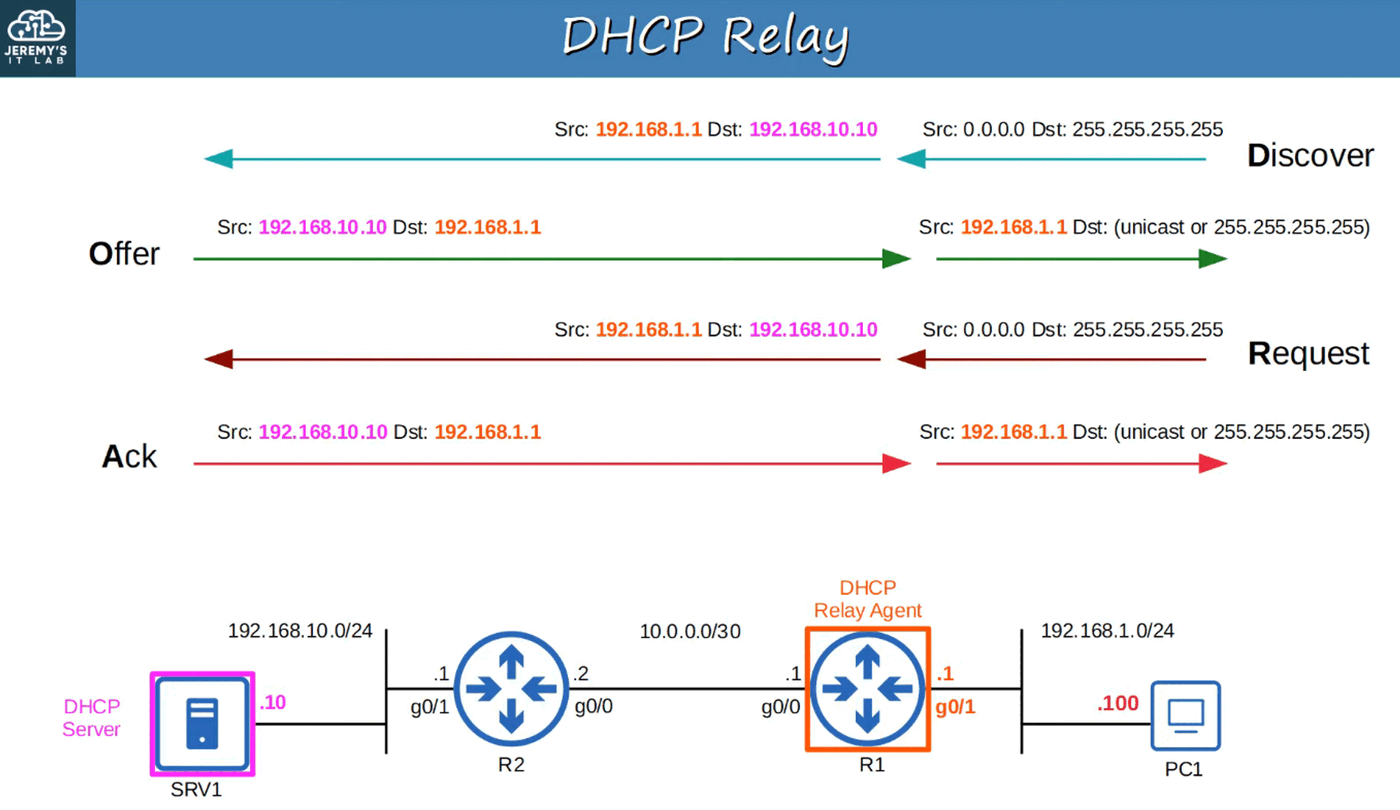
\includegraphics[keepaspectratio,alt={image}]{images/40-dhcp/img-018.png}}
\end{figure}

\section{Configuring DHCP in Cisco
IOS}\label{configuring-dhcp-in-cisco-ios}

Commands for configuring DHCP SERVERS in Cisco IOS

\begin{figure}
\centering
\pandocbounded{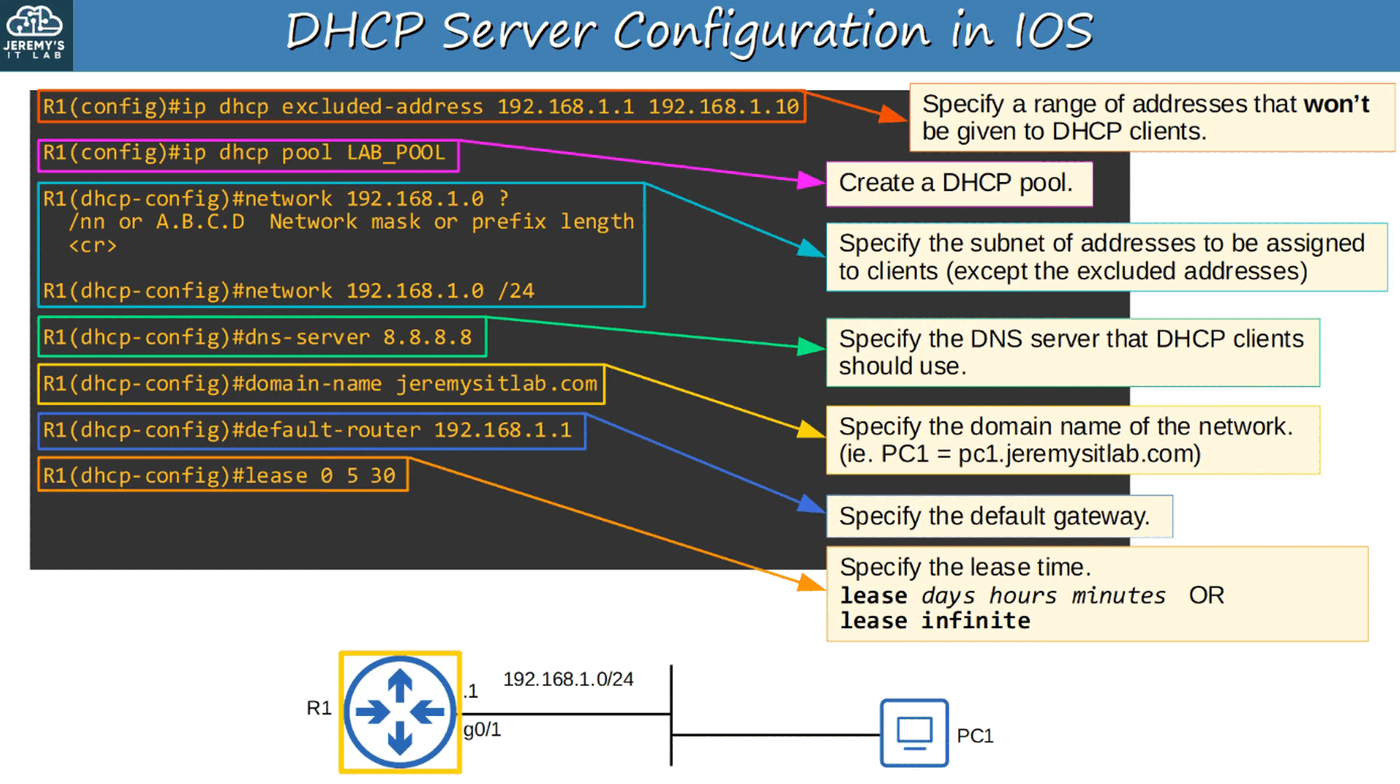
\includegraphics[keepaspectratio,alt={image}]{images/40-dhcp/img-019.png}}
\end{figure}

Command \passthrough{\lstinline!show ip dhcp binding!}

\begin{figure}
\centering
\pandocbounded{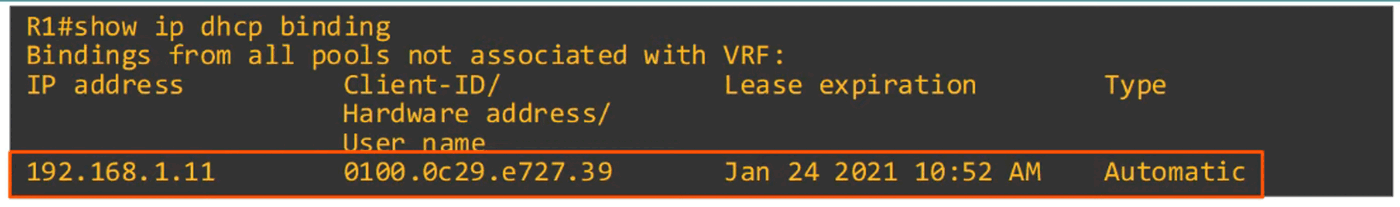
\includegraphics[keepaspectratio,alt={image}]{images/40-dhcp/img-020.png}}
\end{figure}

\begin{figure}
\centering
\pandocbounded{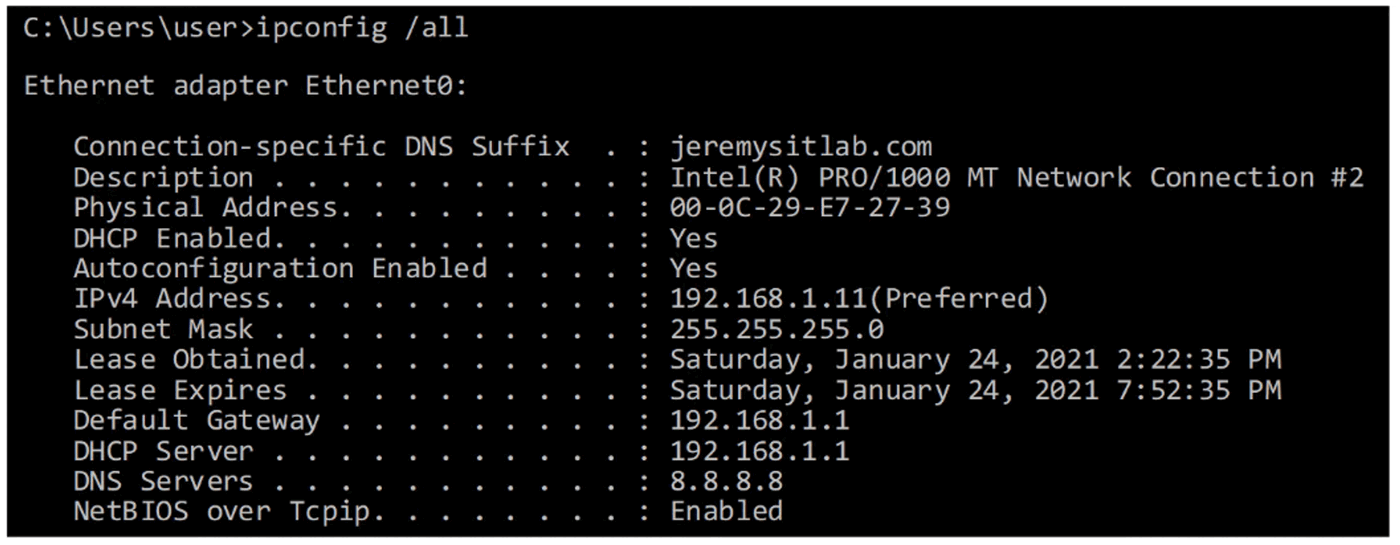
\includegraphics[keepaspectratio,alt={image}]{images/40-dhcp/img-021.png}}
\end{figure}

\section{DHCP Relay Agent Configuration in
IOS}\label{dhcp-relay-agent-configuration-in-ios}

\begin{figure}
\centering
\pandocbounded{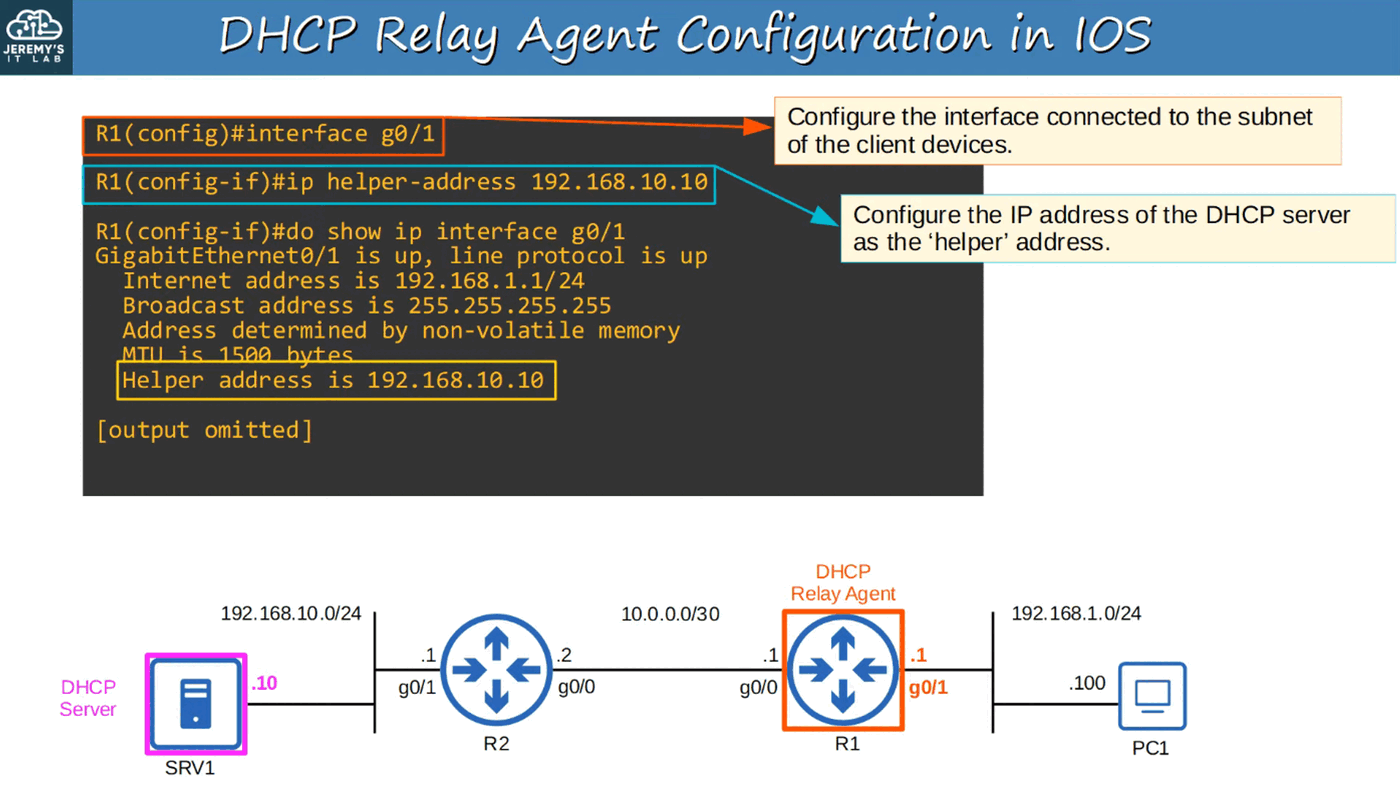
\includegraphics[keepaspectratio,alt={image}]{images/40-dhcp/img-022.png}}
\end{figure}

\section{Relay Agent Must Have Connectivity with DHCP
Server}\label{relay-agent-must-have-connectivity-with-dhcp-server}

\section{DHCP Client Configuration in
IOS}\label{dhcp-client-configuration-in-ios}

\begin{figure}
\centering
\pandocbounded{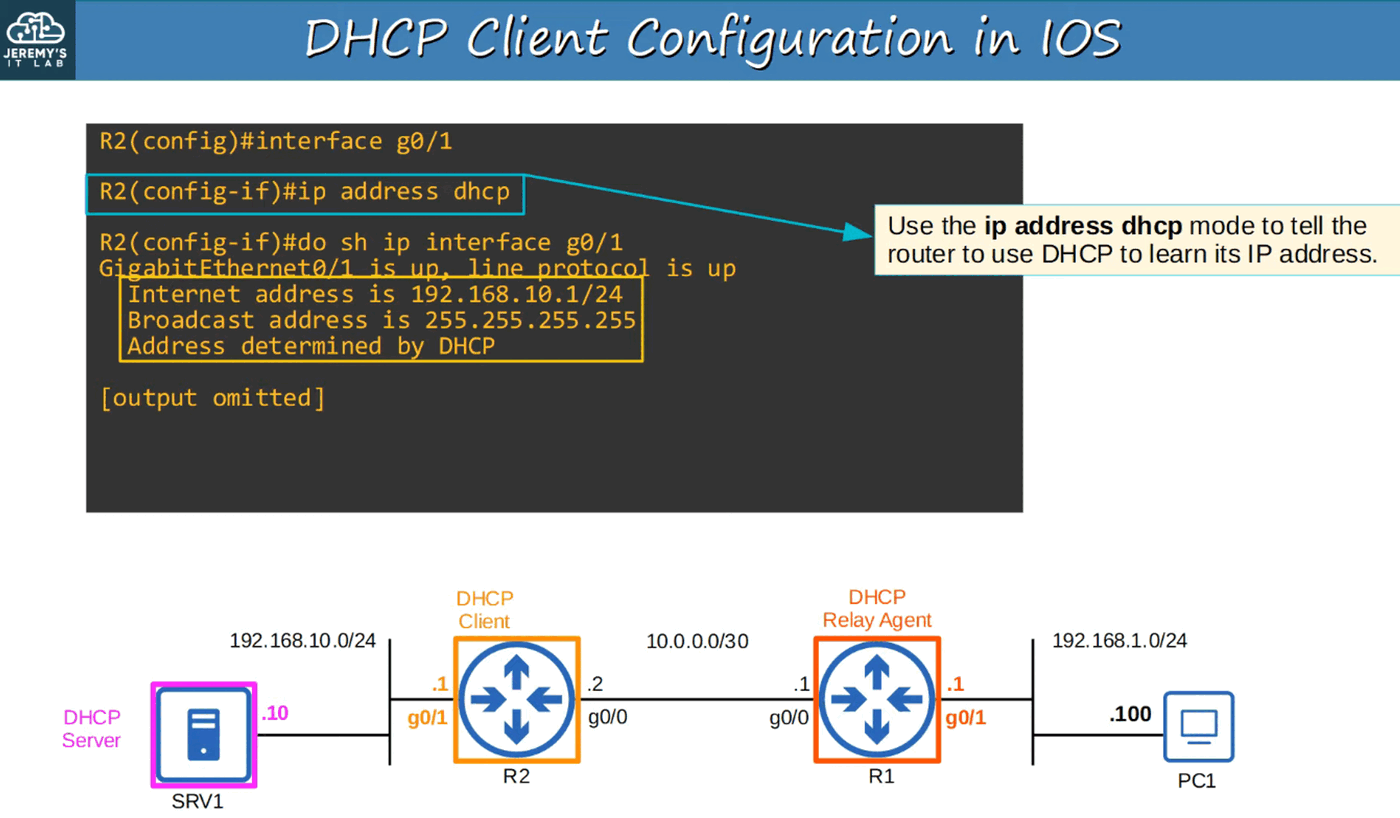
\includegraphics[keepaspectratio,alt={image}]{images/40-dhcp/img-023.png}}
\end{figure}

\section{Commands Summary}\label{commands-summary}

\begin{figure}
\centering
\pandocbounded{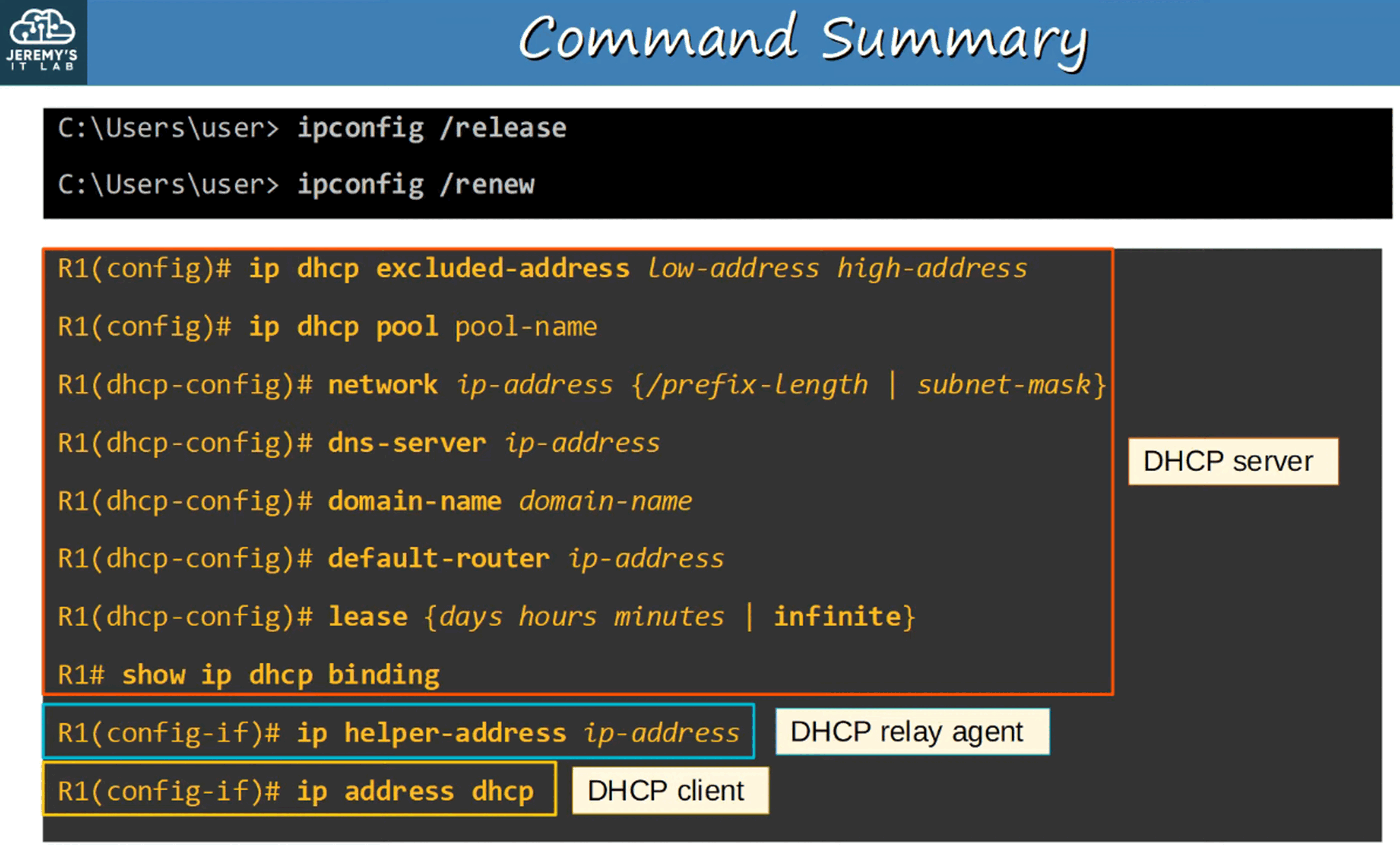
\includegraphics[keepaspectratio,alt={image}]{images/40-dhcp/img-024.png}}
\end{figure}
